\documentclass{mechexpans}
\experimentname{Maxpid Controlled Function Chain}
\author{}
\def\BetaLabel{The rotation of the motor $\beta$(round)}
\def\ThetaLabel{The rotation of the arm $\theta$ \si{\degree}}
\def\XLabel{The position of the nut $x$\si{\mm}}
\def\K{-4}
\def\B{170}
\def\ArctanAB{0.72}
\def\OrderTwoFactor{0.00094}
\def\OrderOneFactor{0.08}
\def\ConstantInsideArcsin{0.66}

\newcommand*{\DataFrom}[1]{Data taken from #1}

\begin{document}
\maketitle
\begin{solution}
  \begin{parts}
    \part The figure 1: Control board, arm, protection casting.
    \part The figure 2: Tachometric generator, motor, screw, nut, angular potentiometer.
  \end{parts}
\end{solution}

\begin{solution}
  \begin{tikzpicture}[scale=0.8]
    \begin{axis}[PlotStyle, xlabel={\BetaLabel}, ylabel={\ThetaLabel},
      title={Input/Output Relation from 0.1.mvt},]
      \addplot+ [mark=none] table [x=Beta, y=Theta,] {./data/0.1.mvt};
    \end{axis}
  \end{tikzpicture}
  \begin{tikzpicture}[scale=0.8]
    \begin{axis}[PlotStyle, xlabel={\BetaLabel}, ylabel={\ThetaLabel},
      title={Input/Output Relation from 0.4.mvt},]
      \addplot+ [mark=none] table [x=Beta, y=Theta,] {./data/0.4.mvt};
    \end{axis}
  \end{tikzpicture}
\end{solution}

\begin{solution}
  The approximative pitch of the screw is 0.400\si{\cm}(4\si{\mm}) and the screw has a right-hand thread.
  The relation is:
  \begin{equation*}
    \Delta x = - p\Delta\beta
  \end{equation*}
  The hypotheses are as follow:
  \begin{itemize}
    \item Suppose the motor rotates clockwise
    \item and the positive part of $x$ axis is along $\vec{x_1}$.
  \end{itemize}
  The known facts are as follow:
  \begin{itemize}
    \item By definition, a right-hand screw is the one that will be loosen when the nut revolves clockwise along it.
    \item In our case, the one that moves respecting to the protection casting is the \emph{screw}, not the nut.
  \end{itemize}
  Thus, when the motor rotates clockwise, the nut moves along the negative part of the $x$.
  The sign of the relation is negative.
\end{solution}

\begin{solution}
  For the pitch we have:
  \begin{equation*}
    p = \abs{\frac{\Delta x}{\Delta\beta}}
  \end{equation*}
  From the linear regression we have $p = 4\si{\mm}$, which matches the measurement.
  \vskip1em
  \begin{tikzpicture}
    \pgfplotsset{%
      legend style={font=\footnotesize}
    }
    \begin{axis}[PlotStyle,
      title={Data taken from 0.4.mvt}, xlabel={\BetaLabel}, ylabel={\XLabel},]
      \addplot+[mark=none] table [x=Beta, y=X] {./data/0.4.mvt};
      \addlegendentry{Measured value}
        \addplot+[mark=none] table[x=Beta, y={create col/linear regression={y=X}}] {./data/0.4.mvt};
        \addlegendentry{%
            $ x = \pgfmathprintnumber{\pgfplotstableregressiona} \cdot \beta
            \pgfmathprintnumber[print sign]{\pgfplotstableregressionb}$ lin. Regression
          }
      \end{axis}
    \end{tikzpicture}
\end{solution}

\begin{solution}
    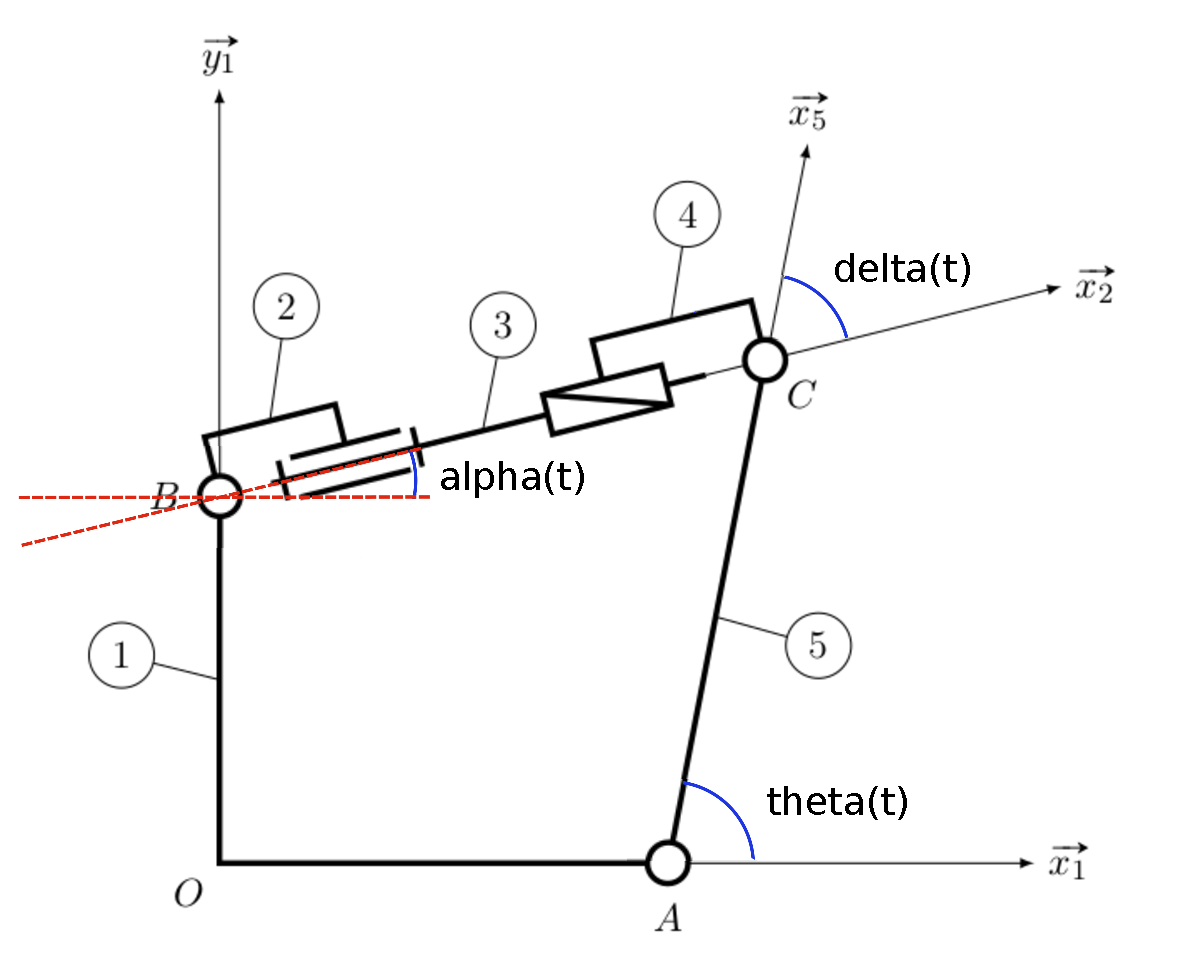
\includegraphics[width=0.6\textwidth]{angular-indicator.eps}

    The angular parameters $\theta(t)$, $\alpha(t)$ and $\delta(t)$ are indicated in the image above.
\end{solution}

\begin{solution}
  \begin{align*}
    a &= 70 \si{\mm} \\
    b &= 80 \si{\mm} \\
    c &= 80 \si{\mm} \\
  \end{align*}
\end{solution}

\begin{solution}
  The input parameter is $\beta(t)$ and the output parameter is $\theta(t)$.
\end{solution}

\begin{solution}
  The loop closure vector relation is:
  \begin{align*}
    \overrightarrow{OB} + \overrightarrow{BC} + \overrightarrow{CA} + \overrightarrow{AO} &= \vec{0} \\
    a\vec{x_1}+c\vec{x_5}-x(t)\vec{x_2}-b\vec{y_1} &= \vec{0} \\
  \end{align*}
  As $\vec{b_1}$ is represented by $\vec{x_1}$ and $\vec{y_1}$, we have two scalar equations:
  \begin{align*}
    a\vec{x_1} \cdot \vec{x_1} + c \vec{x_5} \cdot \vec{x_1} - x(t) \vec{x_2} \cdot \vec{x_1} &= 0 \\
    c\vec{x_5} \cdot \vec{y_1} - x(t)\vec{x_2} \cdot \vec{y_1} -b\vec{y_1}\cdot\vec{y_1} &= 0\\
  \end{align*}
  The final simplified equations are:
  \begin{align*}
    a+c\cos\left(\theta(t)\right) - x(t)\cos\left(\alpha(t)\right) &= 0 \\
    -b+c\sin\left(\theta(t)\right) - x(t)\sin\left(\alpha(t)\right) &= 0 \\
  \end{align*}
\end{solution}

\def\a{\pgfmathprintnumber{\pgfplotstableregressiona}}
\def\b{\pgfmathprintnumber{\pgfplotstableregressionb}}
\def\TheFormula{\theta = -\arcsin\left(\frac{ x^2-a^2-b^2-c^2 }{2c\sqrt{a^2+b^2}} \right) + \arctan\frac{a}{b}}

\begin{solution}
  Eliminating\footnote{Since $t$ is not relevant to the relation between $\theta$ and $\beta$, we omit $t$ in this solution.}
$\alpha$ from the scalar equations using $\sin^2\alpha + \cos^2\alpha = 1$ yeilds:
  \begin{align*}
    x^2 &= 2c(a\cos\theta - b\sin\theta) + a^2 + b^2 + c^2 \\
    x^2 &= 2c\sqrt{a^2+b^2} \sin\left(\theta - \arctan\frac{a}{b}\right)+ a^2 + b^2 + c^2 \\
    \theta &= -\arcsin\left(\frac{ x^2-a^2-b^2-c^2 }{2c\sqrt{a^2+b^2}} \right) + \arctan\frac{a}{b} \\
           &= -\arcsin\left(\frac{ (\K \beta + \B)^2-a^2-b^2-c^2 }{2c\sqrt{a^2+b^2}} \right) + \arctan\frac{a}{b} \\
           &= - \arcsin(\frac{ 16\beta^2-1360\beta+11200 }{17008}) + 41.19 \\
  \end{align*}
\end{solution}

\def\a{70}
\def\b{80}
\def\c{80}
\begin{solution}
  \def\Title{Experiment and Theoretical Plots}
  \begin{tikzpicture}[scale=0.8]
    \begin{axis}[PlotStyle, samples=100, domain=0:25,
      legend pos=outer north east,
      title={\Title},
      xlabel={\BetaLabel}, ylabel={\ThetaLabel},]
      \addplot+[mark=none]{(atan2(\a,\b) - asin(((\K * x + \B)^2 - \a^2 - \b^2 - \c^2)/(2*\c*sqrt(\a^2+\b^2))))};
      \addlegendentry{Theoretical plot}
      \addplot+ [mark=none] table[x=Beta, y=Theta,] {./data/0.1.mvt};
      \addlegendentry{\DataFrom{0.1.mvt}}
    \end{axis}
  \end{tikzpicture}
\end{solution}

\end{document}
